% This must be in the first 5 lines to tell arXiv to use pdfLaTeX, which is strongly recommended.
\pdfoutput=1
% In particular, the hyperref package requires pdfLaTeX in order to break URLs across lines.

\documentclass[11pt]{article}

% Remove the 'review' option to generate the final version.
\usepackage{acl}

% Standard package includes
\usepackage{times}
\usepackage{latexsym}
\usepackage{graphicx}

% For proper rendering and hyphenation of words containing Latin characters (including in bib files)
\usepackage[T1]{fontenc}
% For Vietnamese characters
% \usepackage[T5]{fontenc}
% See https://www.latex-project.org/help/documentation/encguide.pdf for other character sets

% This assumes your files are encoded as UTF8
\usepackage[utf8]{inputenc}

% This is not strictly necessary, and may be commented out,
% but it will improve the layout of the manuscript,
% and will typically save some space.
\usepackage{microtype}

% If the title and author information does not fit in the area allocated, uncomment the following
%
%\setlength\titlebox{<dim>}
%
% and set <dim> to something 5cm or larger.

\title{AdityaPatkar at WASSA 2023 Empathy, Emotion, and Personality Shared Task: RoBERTa-Based Emotion Classification of Essays, Improving Performance on Imbalanced Data}

% Author information can be set in various styles:
% For several authors from the same institution:
\author{Aditya Patkar\textsuperscript{1} \\
       University of Maryland, College Park \\
       \textsuperscript{1}\texttt{apatkar@umd.edu} \ }
% if the names do not fit well on one line use
%         Author 1 \\ {\bf Author 2} \\ ... \\ {\bf Author n} \\
% For authors from different institutions:
% \author{Author 1 \\ Address line \\  ... \\ Address line
%         \And  ... \And
%         Author n \\ Address line \\ ... \\ Address line}
% To start a seperate ``row'' of authors use \AND, as in
% \author{Author 1 \\ Address line \\  ... \\ Address line
%         \AND
%         Author 2 \\ Address line \\ ... \\ Address line \And
%         Author 3 \\ Address line \\ ... \\ Address line}

% \author{First Author \\
%   Affiliation / Address line 1 \\
%   Affiliation / Address line 2 \\
%   Affiliation / Address line 3 \\
%   \texttt{email@domain} \\\And
%   Second Author \\
%   Affiliation / Address line 1 \\
%   Affiliation / Address line 2 \\
%   Affiliation / Address line 3 \\
%   \texttt{email@domain} \\}

\begin{document}
\maketitle
\begin{abstract}
This paper presents a study on using the RoBERTa language model for emotion classification of essays as part of the 'Shared Task on Empathy Detection, Emotion Classification and Personality Detection in Interactions' \citep{barriere2023wassa}, organized as part of 'WASSA 2023' at 'ACL 2023'. Emotion classification is a challenging task in natural language processing, and imbalanced datasets further exacerbate this challenge. In this study, we explore the use of various data balancing techniques in combination with RoBERTa \citep{liu2019roberta} to improve the classification performance. We evaluate the performance of our approach (denoted by adityapatkar on \href{https://codalab.lisn.upsaclay.fr/competitions/11167#results}{Codalab} \citep{codalab_competitions}) on a multi-label dataset of essays annotated with eight emotion categories, provided by the Shared Task organizers. Our results show that the proposed approach achieves the best macro F1 score in the competition's training and evaluation phase. Our study provides insights into the potential of RoBERTa for handling imbalanced data in emotion classification. The results can have implications for the natural language processing tasks related to emotion classification.
\end{abstract}


\section{Introduction}

Emotion detection and classification in natural language processing (NLP) is a crucial task with various applications such as sentiment analysis, recommendation systems, and chat-bots. In recent years, deep learning-based models, particularly those based on transformer architectures, have shown remarkable performance in a range of NLP tasks. Among them, the RoBERTa model has gained significant attention for its superior performance on various metrics.

However, emotion classification is a particularly challenging task, as emotions are subjective and context-dependent, and often manifest in subtle and nuanced ways. Additionally, imbalanced datasets, where certain emotion categories have fewer instances than others, are common in emotion classification tasks, further complicating the task.

We had to work with a highly imbalanced dataset. The task being multi-label added further complexity. Previous works on emotion classification mainly focus on single label classification \citep{barriere2022wassa}, use somewhat balanced dataset \citep{demszky2020goemotions} or work with texts shorter than essays \citep{mohammad-2012-emotional}. The last point is crucial as when working with essays, we have to consider the perceived emotions of the complete essay.

Our proposed system contains a RoBERTa-large model. We will discuss various techniques that we tried to overcome the challenges faced by an imbalanced dataset, biggest of which was over-fitting to the majority label. Some approaches include using paraphrasing to increase the size of the dataset, adding class weights as a feature, weight decay etc.

\section{Dataset}

The dataset provided for the emotion classification task contains essays written in response to news articles where harm to individuals or groups is present. The dataset was divided into training, development, and test sets. Table \ref{tab:data_split} shows the number of samples in each split of the dataset. We focused our analysis on the 'essay' and 'emotion' columns, discarding other columns like gender and age, which were not relevant to the task.

During the exploratory data analysis, we observed that the training and development datasets were comparable in terms of essay length (averaging between 75-80 words per essay) and the split between single-label and multi-label rows. Furthermore, we analyzed the top five most frequent words after removing stop-words in the training dataset, which included 'people,' 'like,' 'feel,' 'think,' and 'sad.' This finding suggests that the essays in the dataset often expressed personal opinions and feelings related to human experiences.

To gain further insights, we also examined the top direct objects of the verb in the sentences for each label. For example, the words 'journey' and 'hardship' were amongst the top 5 most frequent direct objects for the label 'Joy,' while for 'Sadness,' the words 'life' and 'child' were present amongst the top 5. This observation highlights the differences in language use across different emotions and provides clues to the underlying emotional experiences. Our exploratory data analysis sheds light on the characteristics of the dataset and provides valuable insights into the language use associated with different emotions.

One of the major challenges encountered in the emotion classification task was the presence of 'data imbalance'. Also, the emotion column in the dataset allowed for a single essay to have multiple emotions, making the classification task more complex. For instance, an essay could express both 'Disgust' and 'Anger.'

\begin{table}
\centering
\begin{tabular}{lc}
\hline
\textbf{Dataset} & \textbf{Rows}\\
\hline
\verb|Training| & 792 \\
\verb|Development| & 208 \\
\verb|Test| & 100 \\
\hline
\hline
\verb|Total| & 1100
\end{tabular}
\caption{Number of rows in each split of the dataset.}
\label{tab:data_split}
\end{table}


The training dataset exhibited a highly skewed distribution towards 'Sadness' and 'Neutral' emotions, as shown in Table~\ref{tab:emotion_split}. The issue of data imbalance is evident from the fact that our baseline model failed to predict the under-represented emotions, such as 'Joy' and 'Surprise.'

\begin{table}
\centering
\begin{tabular}{lc}
\hline
\textbf{Emotion} & \textbf{Occurrences}\\
\hline
\verb|Sadness| & 383 \\
\verb|Neutral| & 240 \\
\verb|Joy| & 10 \\ 
\verb|Anger| & 124 \\
\verb|Surprise| & 19 \\
\verb|Disgust| & 100 \\ 
\verb|Fear| & 33 \\
\verb|Hope| & 32 \\
\hline
\end{tabular}
\caption{Number of samples for each emotion in the training dataset.}
\label{tab:emotion_split}
\end{table}

In natural language processing tasks, data imbalance is often addressed through under-sampling or oversampling techniques. We implemented a few techniques to address this problem. We will discuss those in the forthcoming sections.

\section{Baseline}

To establish a baseline for our multi-label emotion classification task, we opted to fine-tune the BERT model \citep{devlin2019bert} using the HuggingFace Transformers library \citep{wolf2020huggingfaces}. We detached the head of the model to customize it for our task. For data pre-processing, we retained only the 'essay' and 'emotion' columns as they were relevant for our task. We utilized the 'bert-base-uncased' tokenizer to obtain the final embedding of the essays, which we one-hot encoded for multi-label classification.

We trained the BERT model using TensorFlow, with a learning rate of 2e-05, binary cross-entropy as the loss, and the Adam optimizer. We trained the model for 25 epochs, with a batch size of 16. To prevent over-fitting, we implemented early stopping by monitoring the validation loss. To optimize the threshold on the logits for the labels, we performed a random search. As we trained the model, our training loss kept going down, but after a point, the validation loss did not go down. Instead it increased. This is a sign of overfitting. Figure~\ref{fig:baseline_metrics} shows us how the baseline model performed for each individual label.

\begin{figure}[bhp]
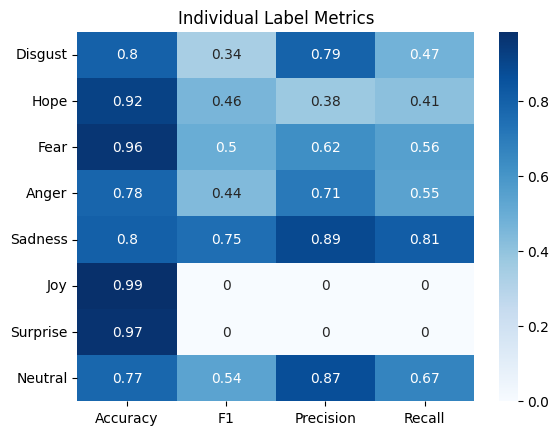
\includegraphics[width=\columnwidth]{BERT_Dev_Metrics.png}
\caption{Individual label accuracy, precision, recall and F-1 score of the baseline model on the development dataset.}
\label{fig:baseline_metrics}
\end{figure}


\section{Proposed Approach}

We introduce a system\footnote{Source code available at \url{https://github.com/adityapatkar/WASSA2023_EMO}} that takes into account the limitations put forward by the data imbalance. We use the 'roberta-large' model with a few tweaks which helped us beat the results of the baseline in every metric.

\begin{figure}[bhp]
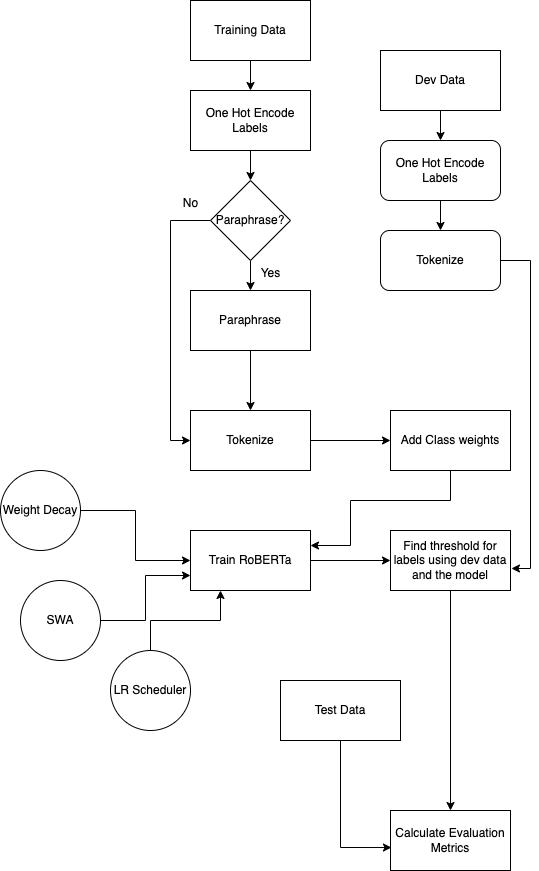
\includegraphics[width=\columnwidth]{flowchart.png}
\caption{High-level flowchart of our proposed system.}
\label{fig:system_chart}
\end{figure}

\subsection{Our System}

\begin{figure}[bhp]
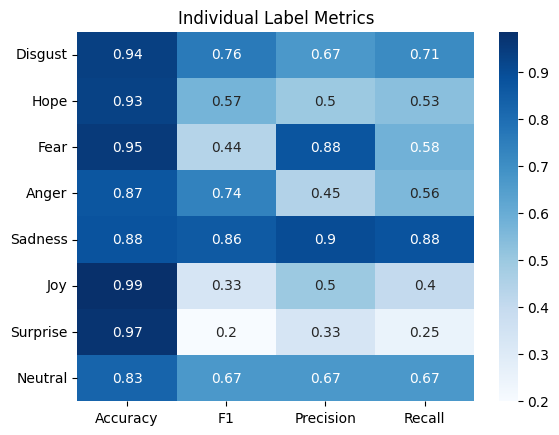
\includegraphics[width=\columnwidth]{roberta_metrics_emo.png}
\caption{Individual label accuracy, precision, recall and F-1 score of our system on the development dataset.}
\label{fig:roberta_metrics}
\end{figure}

Our proposed system deviates from the baseline in several important ways, which we believe have contributed to improved performance on the task at hand.

Firstly, we utilize the RoBERTa model, which has a deeper architecture than the BERT model used in the baseline. This deeper architecture allows for more effective learning of context, which is particularly important for the purpose of this multi-label classification task.

In addition to using a different model architecture, we also implement weight decay to address the issue of over-fitting. This involves setting a defined percentage of weights to exponentially decay to zero, helping to prevent the model from becoming too specialized to the training data. Furthermore, we also implement Stochastic Weight Averaging (SWA) as a means of improving generalization \citep{izmailov2019averaging}. Our implementation of SWA involves modifying the learning rate schedule and averaging weights after each epoch.

One major innovation we introduced was the use of class weights as a feature in the training dataset. By calculating class weights for each essay based on their inverse frequency, we were able to improve the macro F-1 score by 11\%. Specifically, for each class $i$, we calculated the weight $w_i$ as $w_{i} = \frac{n}{k \times n_{i}}$, where $n$ is the total number of samples in the training data, $k$ is the number of classes, and $n_{i}$ is the number of samples in class $i$. These weights were then added to the data as a feature.

Finally, we attempted to augment the dataset size by paraphrasing essays associated with under-represented emotions. However, we found that this approach was not effective, as the model started to over-fit to the training data.

Figure~\ref{fig:system_chart} provides a high-level flowchart of our system, highlighting the key differences from the baseline. Overall, our changes to the system architecture and training approach have led to improved performance on the task at hand.

\begin{table*}
\centering
\subsection*{Development Metrics}
\begin{tabular}{llll}
\hline
\textbf{Model} & \textbf{Macro F-1}\ & \textbf{Macro Recall} & \textbf{Macro Precision}\\
\hline
\verb|DistilBERT| & 0.4021 & 0.3797 & 0.5560 \\
\verb|Baseline BERT| & 0.4409 & 0.4458 & 0.4835 \\
\verb|BERT + Paraphrasing| & 0.4207 & 0.4062 & 0.4614 \\
\verb|BERT + RoBERTa Ensemble| & 0.4251 & 0.3703 & 0.5250 \\
\verb|Proposed System with RoBERTa| & \textbf{0.5790} & \textbf{0.6251} &\textbf{0.5711} \\
\hline
\end{tabular}
\subsection*{Test Metrics}
\begin{tabular}{llll}
\hline
\textbf{Model} & \textbf{Macro F-1}\ & \textbf{Macro Recall} & \textbf{Macro Precision}\\
\hline
\verb|Baseline BERT| & 0.5464 & \textbf{0.7257} & 0.5039 \\
\verb|Proposed System with RoBERTa| &\textbf{0.7012} & 0.6773 & \textbf{0.8105} \\
\hline
\end{tabular}
\caption{Evaluation metrics on the development and test set.}
\label{tab:dev_test_metrics_macro}
\end{table*}



\subsection{Training}

Our system employs the 'roberta-large' model, which was trained for 25 epochs using a learning rate of 2e-5. To avoid over-fitting, we implemented a weight decay of 0.8\%. We also employed the Stochastic Weight Averaging (SWA) technique, which averages the model weights after each epoch, thereby enhancing generalization. We used the Adam optimizer for optimization and binary cross-entropy as the loss function.

\subsection{Evaluation}

Similar to the baseline model, we performed a random search on the logits to determine the best threshold. Our search yielded a value of -0.075 as it maximized the F-1 score on the development set. Figure~\ref{fig:roberta_metrics} displays the performance of our proposed system for each individual label. It is evident that there is an improvement in performance compared to the baseline. Notably, emotions with a low number of samples are now being predicted, which the baseline failed to predict. Table~\ref{tab:dev_test_metrics_macro} compares the results of the baseline and the proposed system on the development set and the test set. Our system shows a considerable improvement in all metrics except the recall over the baseline.

\section{Alternate Approaches}

We employed alternative approaches in our study, in addition to the baseline model. The first approach involved utilizing a DistilBERT model \citep{sanh2020distilbert}, for a strictly single-label classification. The model was trained for 100 epochs with a learning rate of 1e-5. However, the results were unsatisfactory.

In the second approach, we utilized BERT as the underlying model, similar to the baseline approach, but expanded the dataset by paraphrasing essays related to labels with less than 40 samples. However, this approach did not perform better than the baseline, due to overfitting of the training data.

Finally, we had observed that ensemble models had a good performance on emotion classification tasks (\citet{maheshwari-varma-2022-ensemble}, \citet{Ganaie_2022}). We used the PyTorch implementation of RoBERTa and BERT and fine-tuned both models using the binary cross-entropy loss and optimized them using the Adam optimizer with a learning rate of 1e-05. We used the RoBERTa tokenizer for RoBERTa and the BERT tokenizer for BERT to tokenize the input text. After adding the sigmoid head for 8 classes, we trained both models for 40 epochs, with early stopping based on validation loss criteria. For the final prediction, we took the average output probability of the two models and used a threshold of 0.066 to predict the labels. 

Details of the performance of these approaches on the development set can be found in Table \ref{tab:dev_test_metrics_macro}.

\section{Conclusion}

In conclusion, this paper presents a study on using the RoBERTa language model for emotion classification of essays, focusing on addressing the challenges posed by imbalanced datasets. The proposed approach combines various data balancing techniques with RoBERTa to improve classification performance, and the results show that the proposed approach achieved the best macro F1 score in the competition's training and evaluation phase. The study provides valuable insights into the potential of RoBERTa for handling imbalanced data in emotion classification, which can have implications for natural language processing tasks related to emotion classification. Overall, the proposed approach offers a promising direction for future research in this field.

\nocite{buechel-etal-2018-modeling, codalab_competitions, barriere2023wassa, barriere2022wassa, tafreshi2021wassa, omitaomu2022empathic}

\bibliography{anthology,custom}
\bibliographystyle{acl_natbib}

\end{document}
